\documentclass[11pt]{article}
\title{Symmetry 9}
\author{https://github.com/heptagons/lenses}
\date{2024/1/12}

\usepackage{graphicx}

\usepackage[margin=0.75in]{geometry}
\usepackage{float} % {figure}{H}
\usepackage{amsmath} % \dfrac

\begin{document}

\maketitle
\begin{abstract}
Symmetry 9
\end{abstract}

\section{Rhombus}

\section{Lenses}

\subsection{Lenses from stars}

\begin{figure}[h]
\centering
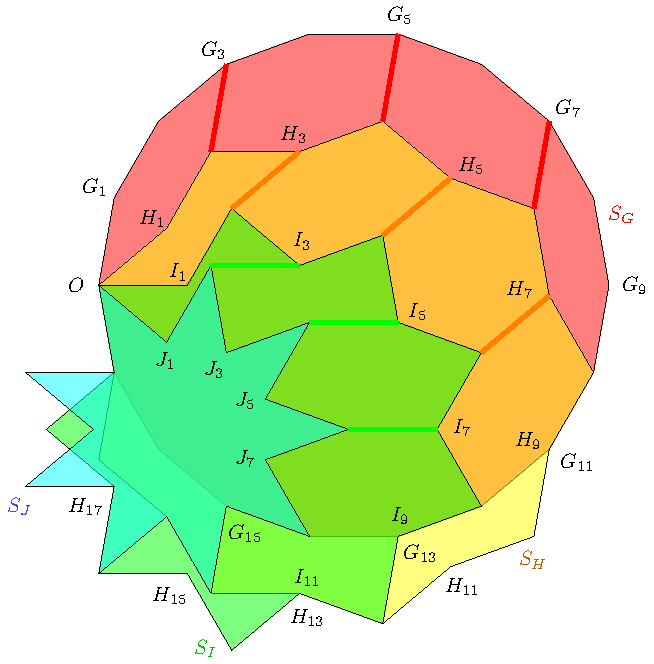
\includegraphics[scale=1]{stars-9}
\caption{Symmetry $9$ stars $\{S_G,S_H,S_I,S_J\}$ dissected with vectors to get symmetry-9 hexagonal lenses.}
\label{fig:stars-9}
\end{figure}

Figure \ref{fig:stars-9} show the disposition of the symmetry $9$ four stars $\{S_G,S_H,S_I,S_J\}$. We denote the $18$ vertices of every star as $\{X_0,X_1,...,X_{17}\}$ where $X = \{G,H,I,J\}$. Only some vertices are labeled in the figure. First we make coincident at vertice $O$ all the vertices $G_0,H_0,I_0,J_0$. With the center at $O$ we rotate star $S_H$ to make coincident vertices $G_{17}$ and $H_{17}$. Similarly we rotate stars $S_I$ and $S_J$ to make coincident vertices $G_{17}$ and $I_{17}$ and vertices $G_{17}$ and $J_{17}$. The rotations also joined another different vertices.

First we add three new edges (in red) joining the stars $S_G$ and $S_H$ vertices: $\overline{G_3H_2}$, $\overline{G_5H_4}$ and $\overline{G_7H_6}$ dissecting the red region into four hexagons, two of them essentially different. The three consective angles of the two hexagons are shown: $(\textbf{1,4,4})$ and $(\textbf{3,4,2})$.

Then we add three new edges (in orange) joining the stars $S_H$ and $S_I$ vertices: $\overline{H_3I_2}$, $\overline{H_5I_4}$ and $\overline{H_7I_6}$ dissecting the orange region into four hexagons, two of them new. The three consective angles of the the two hexagons are show: $(\textbf{1,5,3})$ and $(\textbf{3,3,3})$.

Finally we add three more edges (in green) joining the stars $S_I$ and $S_J$ vertices:
$\overline{I_3J_2}$, $\overline{I_5J_4}$ and $\overline{I_7J_6}$ dissecting the green region into four hexagons, two of them new. The three consective angles of the the two hexagons are show: $(\textbf{1,6,2})$ and $(\textbf{2,5,2})$.

The three consecutive angles of the hexagons are of the form $(a,b,c)$ where $a+b+c = 9$. Table \ref{tbl:hexagons-angles}

\begin{table}[H]
\begin{center}
\begin{tabular}{| c | c c c | l | }
\hline
Hexagon & $\textbf{a}$ & $\textbf{b}$ & $\textbf{c}$ & Details \\ \hline\
$H_9(1,1)$ & 1 & 1 & 7 & self-intersecting \\[1.1ex] \hline
$H_9(1,2)$ & 1 & 2 & 6 & Lense \textbf{\em H$^+$}\\[1.1ex] \hline
$H_9(1,3)$ & 1 & 3 & 5 & Lense \textbf{\em H} \\[1.1ex] \hline
$H_9(1,4)$ & 1 & 4 & 4 & Lense \textbf{\em G} \\[1.1ex] \hline
$H_9(2,2)$ & 2 & 2 & 5 & Lense \textbf{\em J} \\[1.1ex] \hline
$H_9(2,3)$ & 2 & 3 & 4 & Lense \textbf{\em I} \\[1.1ex] \hline
$H_9(3,3)$ & 3 & 3 & 3 & Lense \textbf{\em A} equal to $H_3(1,1)$ \\[1.1ex] \hline
\end{tabular}
\caption{Symmetry $9$ hexagons with angles factors $a \leq b \leq c$.} 
\label{tbl:hexagons-angles}
\end{center}
\end{table}




\end{document}

